% D03-001. DATA-OZZ v2.4.3, f4993e3e...; selected source claims and limits.
\section{Подготовка поднабора осциллограмм однофазных замыканий на землю}
\label{sec:ch3_earth_fault_subset}

Унификация общего набора осциллограмм создаёт основу для дальнейших
исследований, однако для анализа конкретного процесса требуется отобрать
соответствующие записи. Одной из таких задач является изучение однофазных
замыканий на землю в кабельных сетях. В совместной работе по подготовке
этого поднабора использовался исходный массив из 50~765 записей,
описанный ранее в настоящей главе.\footnote{Евдаков А.Е., Филатова Г.А.
Подготовка и анализ набора осциллограмм для исследования однофазных
замыканий на землю в кабельных сетях. Использована версия материала v2.4.3.}
Отбор и последующая ручная проверка рассматривались как самостоятельная
задача подготовки данных, предшествующая статистическому анализу.

Поднабор нужен для изучения перенапряжений по реальным записям
и подготовки материала для последующего распознавания ОЗЗ.
В настоящем разделе рассматриваются порядок его формирования,
распределение зарегистрированных максимумов и условия применения
полученных результатов. Связь ОЗЗ с развитием многофазного повреждения
требует отдельного рассмотрения последовательности событий,
которую одно распределение максимумов не описывает.

\subsection{Отбор и ручная проверка записей}

На первом этапе сигналы приводились к относительным единицам с помощью
коэффициентов нормализации. Для поиска предполагаемых интервалов ОЗЗ
анализировались первые гармоники напряжения нулевой последовательности
и фазных напряжений. Их значения сравнивались с заданными порогами
по амплитуде и длительности. Дополнительно исключались интервалы
со сходными амплитудами напряжений трёх фаз. Такой порядок позволял
выделить кандидатов для дальнейшего просмотра, но сам по себе
не подтверждал наличие ОЗЗ в каждой выбранной записи.

Все отобранные кандидаты проверялись вручную. При просмотре исключались
записи, ошибочно принятые за ОЗЗ, уточнялись границы процесса
и оценки перенапряжений. Максимальное относительное фазное напряжение
рассматривалось в выделенной зоне ОЗЗ. Коммутационные броски при
ликвидации повреждения, находившиеся за её пределами, в эту оценку
не включались. Поэтому исследуемый максимум не следует отождествлять
с максимальным напряжением всей осциллограммы.

\begin{table}[htbp]
\centering
\caption{Распределение кандидатов и проверенного поднабора по кратности перенапряжения}
\label{tab:ch3_earth_fault_selection}
\begin{tabular}{|c|r|r|}
\hline
Кратность & До ручной проверки & После ручной проверки \\
\hline
$<1{,}2$ & 484 & 10 \\
$1{,}2\ldots1{,}71$ & 401 & 83 \\
$1{,}71\ldots1{,}75$ & 37 & 17 \\
$1{,}75\ldots2$ & 550 & 403 \\
$2\ldots2{,}5$ & 318 & 286 \\
$2{,}5\ldots3$ & 45 & 31 \\
$3\ldots3{,}5$ & 0 & 0 \\
$3{,}5\ldots4$ & 8 & 0 \\
$4\ldots4{,}5$ & 18 & 0 \\
$4{,}5\ldots5$ & 4 & 0 \\
$>5$ & 0 & 0 \\
\hline
Всего & 1865 & 830 \\
\hline
\end{tabular}
\end{table}

В таблице~\ref{tab:ch3_earth_fault_selection} подсчитаны осциллограммы,
распределённые по диапазонам максимальной кратности перенапряжения
в выбранных зонах. Сумма строк до ручной проверки составляет 1865,
после неё в поднаборе остаются 830 записей.\footnote{В тексте и итоговой
строке исходной статьи указано 1866 кандидатов. Сумма её одиннадцати
числовых строк равна 1865. Для диссертации принято значение,
подтверждённое суммированием; исходное расхождение сохранено.}
При уточнении границ и напряжений запись могла перейти в другой
диапазон. Разность численностей отдельной строки поэтому не является
самостоятельной оценкой числа ошибок алгоритма. Итоговые 830 записей
также не характеризуют полноту поиска всех ОЗЗ в исходном архиве,
поскольку весь массив не проверялся вручную на отсутствие этих процессов.

При интерпретации результатов необходимо учитывать ограничения
измерительных цепей. Нелинейность трансформаторов напряжения и
ограничение диапазона регистрации могут изменять форму сигнала
и занижать зарегистрированные пики. Неисправность измерительной цепи
может, напротив, создавать завышенные значения, не соответствующие
напряжению исследуемого сетевого процесса. Вследствие этого одного
численного максимума недостаточно для подтверждения физического
смысла записи. Ручная проверка дополняет расчёт рассмотрением
формы сигналов и последовательности событий.

Происхождение исходных записей также влияет на состав поднабора.
Осциллограммы, зарегистрированные устройствами БАВР, смещают его
в сторону повреждений, которые развиваются в многофазные короткие
замыкания. Такой материал полезен для изучения последовательности
аварийного процесса, но его распределение нельзя автоматически
распространять на все ОЗЗ в сети. Наличие отдельных развивающихся
повреждений не устанавливает вероятность их перехода в КЗ
и не подтверждает готовый метод прогнозирования.

Полученный поднабор позволяет перейти от общей подготовки данных
к исследованию зарегистрированных перенапряжений и сложностей
распознавания ОЗЗ. Эти задачи отличаются от определения направления
мощности и применимости РНМ. Для проверки соответствующих органов
необходимы собственные целевые состояния и отдельные условия оценки.

\subsection{Распределение зарегистрированных перенапряжений}
\label{sec:ch3_earth_fault_statistics}

Статистический анализ поднабора выполнен в совместной работе,
посвящённой перенапряжениям при ОЗЗ.\footnote{Совместная работа
Евдакова А.Е., Филатовой Г.А. и Яблокова А.А. по статистическому
анализу перенапряжений при однофазных замыканиях на землю.
Использована версия материала v2.3.2 с комментариями.}
Единицей расчёта служила осциллограмма. Для каждой записи использовалась
максимальная кратность напряжения неповреждённых фаз в выделенной
зоне ОЗЗ относительно номинального фазного напряжения.
Эта величина характеризует зарегистрированный максимум и отличается
от действующего значения напряжения или амплитуды первой гармоники,
использованной при предварительном поиске процесса.

Числовые результаты проверены по сохранённой таблице ручного просмотра
v1.7 (Примечание автора: Эмм… А разве это уместно в диссертации, разве здесь есть этот номер v1.7? 
Если нет, то прост убери его описание вообще. Но я могу и ошибаться. 
Если он внутренний, можно примечанием, для нас оставить. 
Как я раньше делал свои комментарии с полезными ссылками. 
А в итоговой версии, это удаляется и в основном тексте отсутствует. 
Ну либо как-то иначе обыграть, а то эта цифра из ниоткуда по сути). 
В расчёт включены 830 записей с отметкой принятия.
Их распределение по диапазонам совпадает с последним столбцом
таблицы~\ref{tab:ch3_earth_fault_selection}, а все девять показателей
описательной статистики совпадают со статьёй в пределах округления.
(Примечание автора: Подожди подожди не надо писать о статье как о чём-то чужом. 
Это моё и есть, как и все остальные. Да, можно делать ссылку на статью, а тут чуть иначе писать, 
но не надо писать что-то вроде «проверили данные, совпадают», то что берётся из статей – 
прям факт, ну может и поправили его, но не надо на этом делать акценты, прост более современные факты будут и всё. 
Касается как текущих вставок, так и всех остальных и других частей текста, можешь прям в инструкцию это.)
Полный список кандидатов в этой версии таблицы содержит 1855 строк
и отличается от ранее приведённого среза отбора. 
(Примечание автора: И тут не надо такого, прост новые цифры, 
а то, что разнятся, можешь примечанием нам, не более. Мы не сравниваем работы, мы вставляем более актуальные их версии.)
Поэтому совпадение
результатов для принятого поднабора не означает совпадения всех
промежуточных версий кандидатов.

\begin{table}[htbp]
\centering
\caption{Описательная статистика максимальной кратности перенапряжения в поднаборе ОЗЗ}
\label{tab:ch3_earth_fault_statistics}
\begin{tabular}{|l|r|}
\hline
Показатель & Значение \\
\hline
Число записей & 830 \\
Среднее & 1,960 \\
Медиана & 1,926 \\
Выборочное стандартное отклонение & 0,274 \\
Выборочная дисперсия & 0,075 \\
Минимум & 0,862 \\
Первый квартиль & 1,823 \\
Третий квартиль & 2,099 \\
Максимум & 2,843 \\
\hline
\end{tabular}
\end{table}

Для расчёта выборочной дисперсии и стандартного отклонения использован
знаменатель $n-1$, где $n=830$. Квартили рассчитаны с линейной
интерполяцией между соседними значениями упорядоченного ряда.
Сохранённые кратности заданы с тремя знаками после запятой.
Повторный расчёт проверяет статистику этой таблицы, но не заменяет
повторного определения максимумов по исходным сигналам.

На рисунке~\ref{fig:ch3_earth_fault_histogram} представлено распределение
записей по кратности перенапряжения. Гистограмма построена заново
(Примечание автора: нафиг вот эти слова «заново».)
по проверенным значениям с одинаковой шириной интервала 0,1.
Она показывает концентрацию записей около двух относительных единиц
при наличии менее многочисленных значений по обе стороны этой области.
Среднее несколько выше медианы. Расстояние между квартилями
составляет около 0,276 и характеризует центральную половину
упорядоченного ряда. Квартильный интервал не задаёт диапазон
наиболее вероятных значений и не выделяет отдельный физический режим.

\begin{figure}[htbp]
\centering
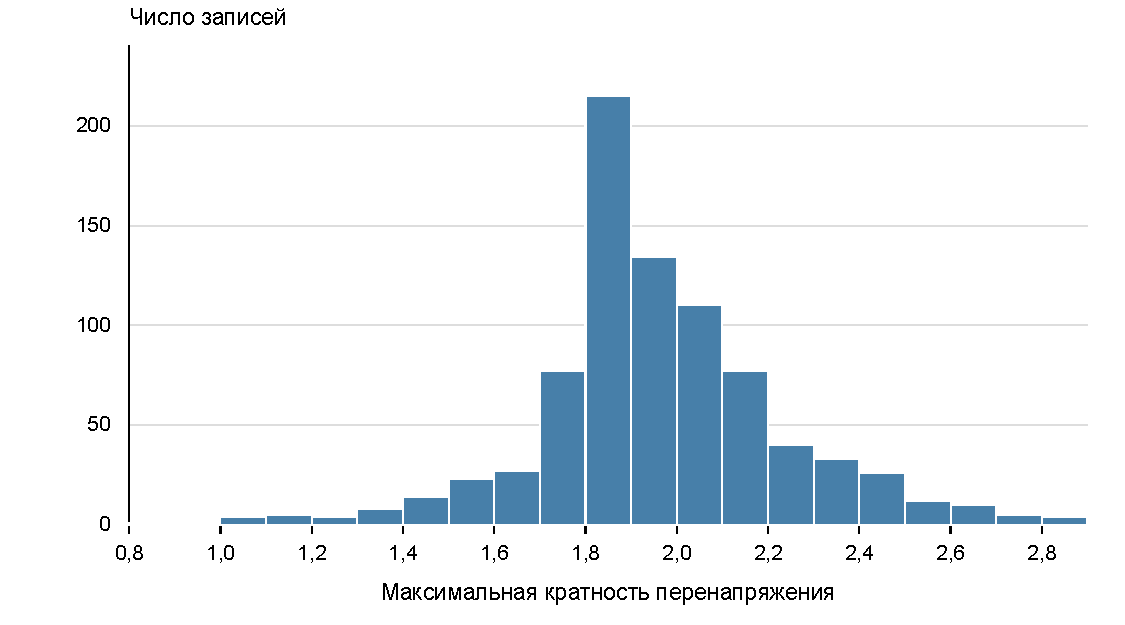
\includegraphics[width=0.94\textwidth]{figures/ozz_overvoltage_histogram.pdf}
\caption{Распределение 830 записей ОЗЗ по максимальной кратности перенапряжения. Ширина интервала равна 0,1}
\label{fig:ch3_earth_fault_histogram}
\end{figure}

Накопленная доля записей показана на
рисунке~\ref{fig:ch3_earth_fault_cdf}. Для выбранной границы она
равна отношению числа максимумов, не превышающих эту границу,
к общему числу принятых записей. График построен ступенчато,
без сглаживания. Он позволяет оценить долю записей ниже заданной
кратности непосредственно по наблюдаемым значениям.

\begin{figure}[htbp]
\centering
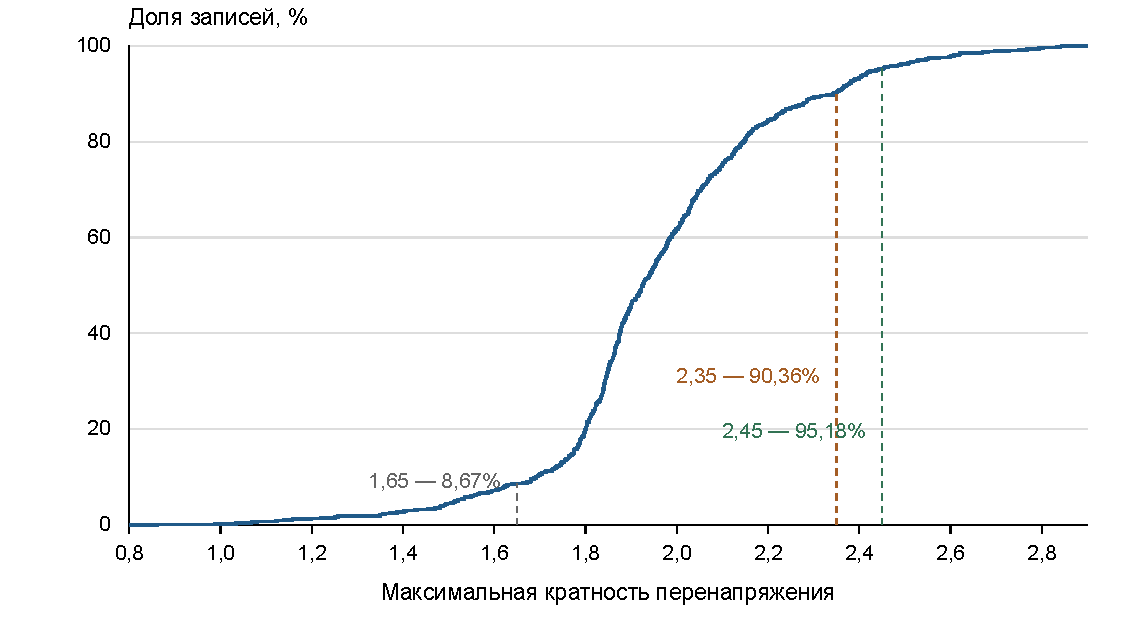
\includegraphics[width=0.94\textwidth]{figures/ozz_overvoltage_cdf.pdf}
\caption{Накопленная доля записей ОЗЗ в зависимости от максимальной кратности перенапряжения}
\label{fig:ch3_earth_fault_cdf}
\end{figure}

Кратность не выше 1,65 имеют 72 записи, что составляет 8,67\%
поднабора. Для границы 2,35 таких записей 750, или 90,36\%,
а для границы 2,45 их число достигает 790, или 95,18\%.
В интервал от 1,65 до 2,35 включительно попадают 678 записей,
или 81,69\%. Таким образом, доля ниже верхней границы и доля
внутри ограниченного с двух сторон интервала имеют разные значения.
Указанные в исходной статье 90\% для этого интервала не подтверждаются
сохранёнными числовыми данными.
(Примечание автора: нафиг вот эти слова «исходной статьи», мы делаем более актуальное. 
Да и странно, что не сходится, на самом деле, очень странно, данные ведь те же самые. 
Вот обдумай и перепроверь всё это, и скажи, где в старом коде косяки. 
И кстати, если есть функции и код построения чего-то в старых разделах для статей,
то не надо прям для каждого графика лепить их тут новые. Надо бы делать систему единой, если много откуда идёт 
– то выносить на уровни выше как-то, в общие инструменты… 
А то я смотрю, много разных функций уже добавила и это надо бы обдумать. Ведь много где начнёт копиться.)

\subsection{Применение результатов и границы исследования}

Полученные характеристики дают количественное описание
зарегистрированных перенапряжений в подготовленном поднаборе.
Они полезны при выборе реальных примеров для анализа сигналов
и сопоставления с результатами моделирования. При этом сравнение
требует одинакового определения напряжения, рассматриваемой зоны
и условий регистрации. Крупные и малые значения после ручной
проверки сохранены в расчёте. Само удаление от основной массы
наблюдений не является основанием исключать запись.

Наблюдаемый максимум 2,843 относится к этим 830 осциллограммам.
Он не устанавливает наибольшее физически возможное перенапряжение
и не исключает более высоких значений при других условиях ОЗЗ.
Состав архива, отбор записей и свойства измерительных цепей
ограничивают перенос результатов на другие сети. Кроме того,
разные файлы не обязательно соответствуют независимым повреждениям.
Поэтому приведённые доли описывают записи поднабора,
а не вероятность возникновения соответствующего режима в сети.

Статистика зарегистрированных максимумов сама по себе не задаёт
уставки защиты по напряжению и не обосновывает изменение требований
к изоляции оборудования. Для применения в конкретном устройстве
нужны его измеряемая величина, условия работы и отдельная проверка.
Для исследований БАВР поднабор представляет интерес прежде всего
как материал для анализа аварийных последовательностей и проверки
распознавания ОЗЗ. Переход от такого распознавания к оценке развития
повреждения требует временной разметки и самостоятельного протокола
испытаний.
